\begin{figure*}
    \centering
    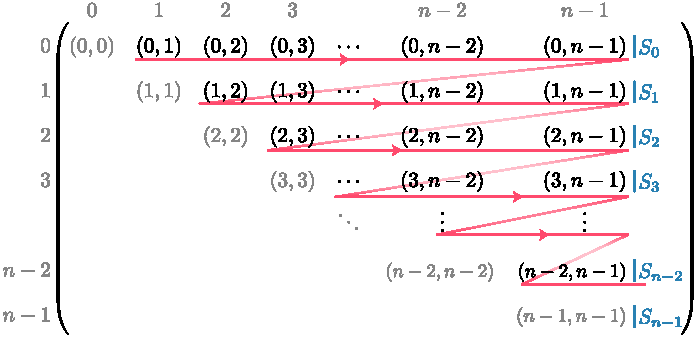
\includegraphics[width=0.78\textwidth]{assets/illustrator/traverse-schema.pdf}
    \caption{Row-major traversal of the adjacency matrix. $n$ is the total number of words (\ie nodes).}
    \label{fig:traverse-schema}
\end{figure*}

\section{Data Preparation}
\label{sec:data}

We use the \href{https://github.com/frodonh/french-words}{\textbf{french-words}} dataset (frodonh, 2020), which contains 691,969 French words. It is compiled from several sources including (among others) the Debian package \href{https://packages.debian.org/fr/sid/wfrench}{wfrench} (used for spell checking), \href{http://www.lexique.org/}{Lexique 3.83} (Boris New \& Christophe Pallier), the \href{https://infolingu.univ-mlv.fr/DonneesLinguistiques/Dictionnaires/telechargement.html}{DELA dictionary} from the University of Marne-la-Vallée as well as the \href{https://github.com/hbenbel/French-Dictionary}{French-Dictionary} (Hussem Ben Belgacem). The words also include \acrfull{pos} tagging information, \eg whether it is a noun, verb, adjective, preposition etc. It also comprises the usage frequency according to Lexique.org and Google Ngrams. We use the average of both sources (or just one if the other is missing).

Since the french-words dataset does not include the phonetic transcriptions, we consult the \href{https://github.com/DanielSWolf/wiki-pronunciation-dict}{\textbf{wiki-pronunciation-dict}} (Daniel Wolf, 2021) extracted from the French \href{https://fr.wiktionary.org/}{Wiktionnaire}. We merge both datasets to obtain 611,786 words with their \gls{ipa} transcription. If multiple phonetic transcription are available, we only store the first one. For easy access, we store the data in a dataclass and serialize it to a pickle file of around \qty{60}{\mega\byte}.

Additionally, we extract all used phonetic symbols and assign integer IDs to them. This enables us to store the transcription as a list of integers. For our examples, we obtain \autoref{tab:phonetic-encoding}. The Needleman-Wunsch algorithm will then work on these integer lists. Note that we consider \textipa{/dZ/} as one symbol, even though it is a combination of \textipa{/d/} and \textipa{/Z/}. The same applies to \textipa{/tS/}. This is to account for the different pronunciation of the combined symbols compared to the individual ones.

% \vspace{-0.2em}

\begin{table}[H]
    \centering
    \begin{tabular}{lll}
    \toprule
    \textbf{Word} & \textbf{\acrshort{ipa}} & \textbf{Encoding} \\
    \midrule
    \textit{puissance} & \textipa{/p\textturnh is\~As/} & $[0,18,16,11,26,11]$ \\
    \textit{nuance} & \textipa{/n\textturnh\~As/} & $[29,18,26,11]$ \\
    \bottomrule
    \end{tabular}
    \caption{Example of two words with their phonetic transcription and encoding.}
    \label{tab:phonetic-encoding}
\end{table}
